
% Appendix Template
\chapter{Sequential eSNN Architectures for Cyber Fraud Detection}
\label{app:eSNN_cyber}

The sequential eSNN classifier is inspired by the architecture proposed in \citep{dora2015sequential}. The proposed architecture is a two layer fully connected feed-forward network as shown in \figurename \ref{fig:esnn}. The input layer consists of $m$ input neurons that convert real-valued inputs to spike-patterns (\figurename \ref{fig:esnn_input}) and the output layer consist of spiking neurons (\figurename \ref{fig:esnn_output}), The network consists of a decision block which monitors the output of the intermediate neurons to determine the predicted class for the presented sample. The intermediate neurons are modelled as IF neurons. These neurons can generate multiple spikes. The intermediate neurons process the input spike patterns from the input neurons. Each intermediate neuron is associated with a particular class and this association is stored in the decision block. The decision block identifies the intermediate neuron that fires first and returns its associated class label as the predicted class label. It should be noted here that although, an intermediate neuron can generate multiple spikes,the decision block uses only the first spike to determine the predicted class. 

\begin{figure}
	\centering
	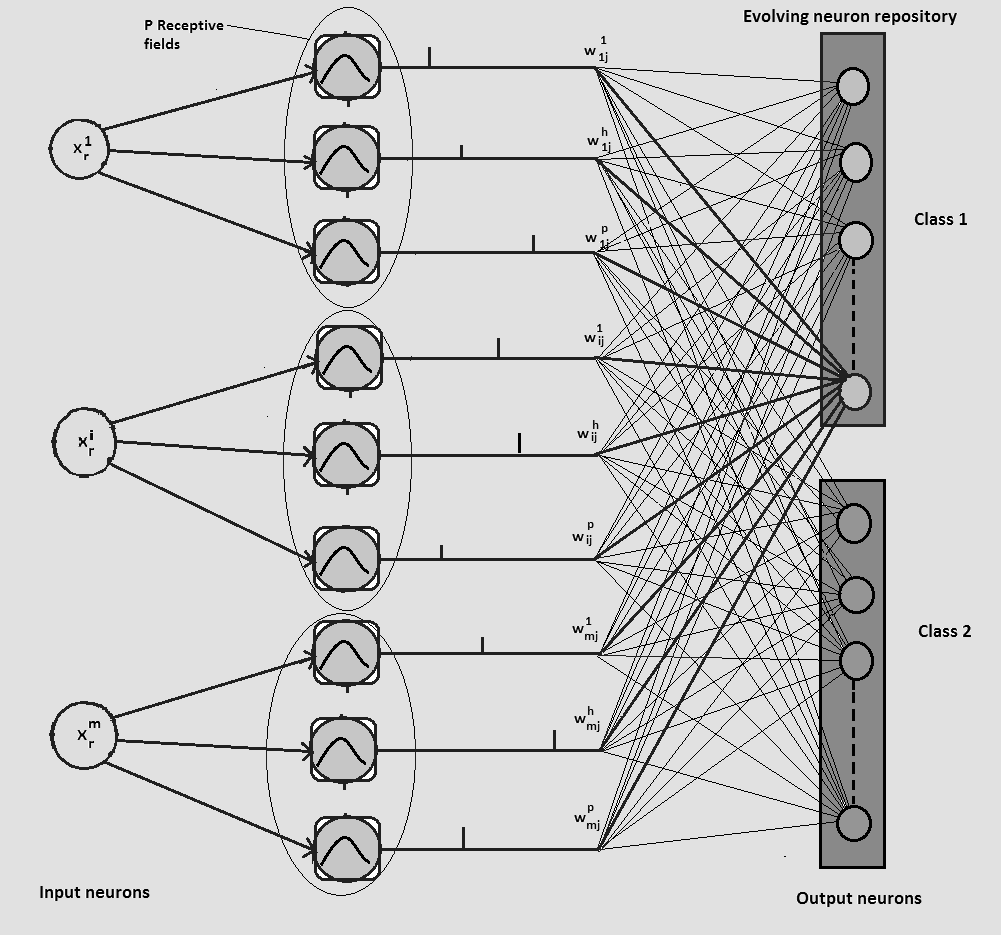
\includegraphics[scale=0.3]{fig/snn/esnn.png}
	\caption{Proposed eSNN architecture for phishing website classification problem.}
	\label{fig:esnn}
\end{figure}

\begin{figure}[!htb]
	\minipage{0.5\textwidth}
	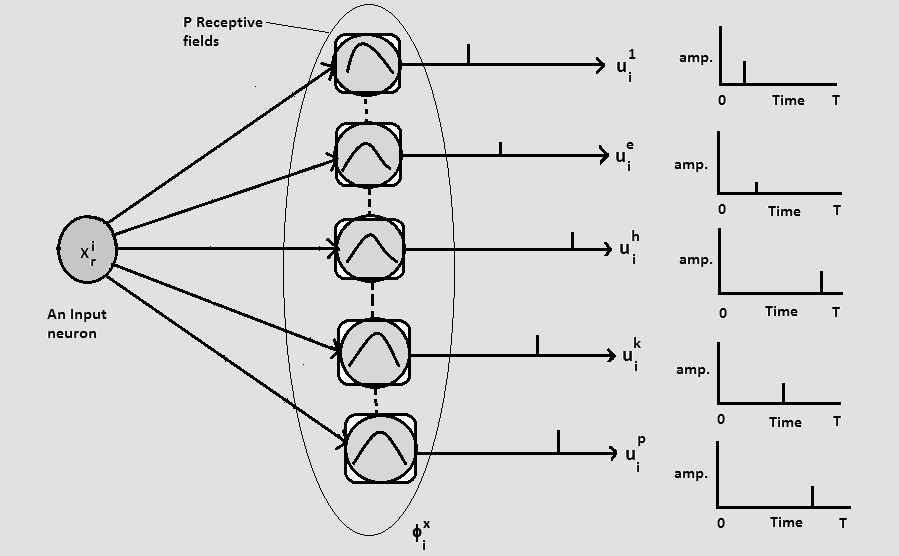
\includegraphics[width=\linewidth]{fig/snn/esnn_input.png}
	\caption{Input neuron model}\label{fig:esnn_input}
	\endminipage\hfill
	\minipage{0.48\textwidth}%
	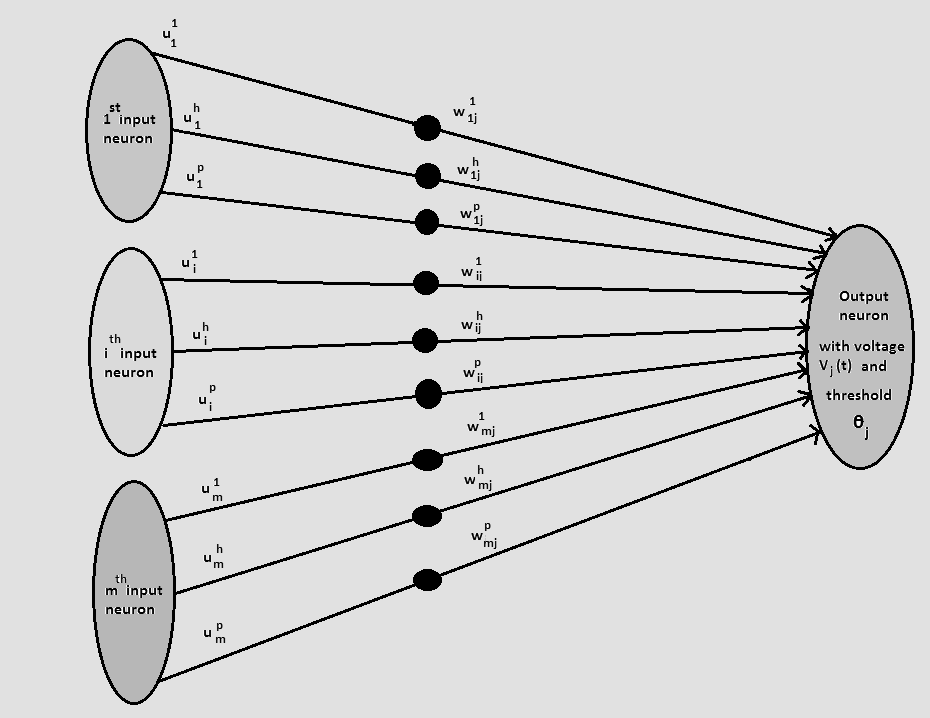
\includegraphics[width=\linewidth]{fig/snn/esnn_output.png}
	\caption{Intermediate neuron model}\label{fig:esnn_output}
	\endminipage
\end{figure}

The proposed method is based on the evolving spiking neural network model for classification. It builds on the Thorpe’s model \citep{thorpe2001spike}, in which early spikes are given more importance. Thorpe's model is highly influenced by the visual pattern recognition system. This method has fast supervised one pass learning. The eSNN have two layers:(1) an input layer and (2) an output layer. Initially, the output layer is empty. The output neurons are added to the output layer depending on the input samples during the training phase.

To deal with real-valued data sets, each data sample needs to map with the sequence of spikes using a precise neural encoding technique. Rank order population encoding is used for this purpose. The population encoding uses the Gaussian receptive fields (GRF) to encode the real-valued data. In this method, each input goes through a fixed number of GRF, and it generates a peak at the certain point of time. Following steps are performed during the classification process:

In rank order coding, every input is encoded individually using a set of $P$ responders (\emph{i.e.} receptive fields). For $i^{th}$ input neuron with $P$ receptive fields $(P>2)$ whose input feature varies from $I^i_{min}$ to $I^i_{max}$. The centre and width of the $h^{th}$ receptive field is given by:

\begin{equation}
	\mu_i^h=I_{min}^i+\frac{(2h-3)}{2}\frac{(I_{max}^i-I_{min}^i)}{(P-2)}
\end{equation}
and
\begin{equation}
	\sigma_i^h=\frac{1}{\gamma}\frac{(I_{max}^i-I_{min}^i)}{(P-2)}
\end{equation} 

where $\gamma$ directly controls the width of the receptive field. The width controls the overlap between the two receptive fields. The $\tau_i^h$ is the firing time of the neuron calculated using:

\begin{equation}
	\tau_i^h=\floor*{T(1-\phi^h_i)}
\end{equation}

Where $T$ is the simulation interval and $\phi^h_i$ is the GRF output defined as follows:

\begin{equation}
	\phi_i^h=\exp(-\frac{(x_r^i-\mu_i^h)^2}{2(\sigma_i^h)^2})
\end{equation}

The output of the $h^{th}$ responder of the $i^{th}$ input neuron is given by:

\begin{equation}
	u_i^h(t, x_r^i)=f_i^h(x_r^i)\delta_i^h(t-\tau_i^h)
\end{equation}

Where $f_i^h(\cdot)$ is the spike amplitude function and $\delta_i^h(.)$ is the dirac delta function or firing time function.

The amplitude of the spikes 
\begin{equation}
	f_i^h(x_r^i)-\frac{\lambda^{r_i^h}}{1+|x_r^i-\mu_i^h|} 
\end{equation}

Where $r_i^h$ is the rank of the $h^{th}$ responder of $i^{th}$ neuron and $\lambda$ is the slope of the amplitude function. The rank of the spikes is determined using the ranking function as follows:


\begin{equation}
	F_R(x, y)=\left\{
	\begin{array}{@{}ll@{}}
	1, & \text{if}\ \phi_i^x\geq \phi_i^y \\
	0, & \text{otherwise}
	\end{array}\right.
\end{equation}

Where $x$ and $y$ are the indices of any two receptive fields of the $i^{th}$ neuron is given by:

\begin{equation}
	r_i^h=1+\sum_{y=1, y\neq h}^P F_R(h,y)
\end{equation}

The equations above describes the spike generation process using the population encoding framework and forms the first layer. The second layer also known as the output layer consists of another set of neurons and next, we describe the rules for the establishment of the synaptic connection between the input and output neuron and synaptic weight initialisation scheme. It is a sequential learning architecture that starts with no output neuron. The algorithm either chooses to add the new neuron at output layer or update the synaptic weight for training sample. 

\begin{itemize}
	\item Addition of output neuron: output neuron addition strategy to evolve the neuron if the current sample satisfies the following condition: 
	\begin{equation}
		\hat{c}= \{\phi\}\ OR\ (c \notin c_{overall})\ OR\ (c \neq \hat{c}\ AND\ ||f-w_{nrs}||>\beta_a)
	\end{equation}
	Where $nrs$ is nearest output neuron of same class, $\beta_a$ is distance threshold constant. $f$ is the set of current sample spike-amplitude-response and $w_{nrs}$ is the existing weight of synapse of the same class in the network. $\phi$ represents for the current sample none of the output neurons fired. coverall is the class label associated with the current output layer neurons and $c$ is the actual class label input training sample. The nearest output neuron is evaluated using the Euclidean distance between the current sample amplitude response and existing synaptic weight of all the output neurons of the same class. If the new sample satisfies the above condition then new output $(k+1)$ neuron is added its synaptic weight and threshold is given as:
	\begin{equation}
		w_{k+1}=f
	\end{equation}
	\begin{equation}
		\theta_{k+1}=\alpha w^T_{k+1} w_{k+1}
	\end{equation}
	
	\item In this strategy, the training sample associated class is not the same as the class associated with the fired output neuron. It means the different class label neuron fire first ($nrl$) and there exists another nearest output neuron of the same class ($nrs$). So the weight vector of different classes associated with output neurons is conflicting in nature. To detect this conflict problem following condition should be satisfied:

	\begin{equation}
		c\neq \hat{c}\ AND\ ||f-w_{nrs}||<\beta_a
	\end{equation}
	To resolve this conflict, the nearest neuron of the same class goes into long-term potentiation and the output neuron goes into different class goes into long-term depression. The synaptic weight update is as follows:
	\begin{equation}
		w_{nrs}=(1-\eta_{nrs})w_{nrs}+\eta_{nrs}f
	\end{equation}
	\begin{equation}
		\theta_{nrs}=(1-\eta_{nrs})\theta_{nrs}+\eta_{nrs}\alpha f^T f
	\end{equation}
	Where $\eta_{nrs}$ is self-adaptive learning factor. It is also called self-adaptive potentiation factor of output neuron. The factor $\eta_{nrs}$ for output neuron given as:
	
	\begin{equation}
		\eta_{nrs}=\frac{\eta_{nrs}}{1+\eta_{nrs}}
	\end{equation}
	The output neuron of the other class goes to long-term depression. Due to the effect of this, the output neuron will not fire for the similar samples and the weights are updated as follows:
	\begin{equation}
		w_{nrl}=(1+k)w_{nrl}-kf
	\end{equation}
	Where $k$ is the depression factor, which controls the synaptic weight depression factor. It is close to zero because the higher value of $k$ results in a massive shift in the synaptic weight. Resulting information loss is stored in the network.
	
	\item Synaptic weight update approach: If the actual class label $c$ is same as the class label associated with the fired output neuron then the synaptic weight of connection and threshold of the output neuron are updated as following:

	\begin{equation}
		w_{nrs}=(1-\eta_{nrs})w_{nrs}+\eta_{nrs}f
	\end{equation}
	\begin{equation}
		\theta_{nrs}=(1-\eta_{nrs})\theta_{nrs}+\eta_{nrs}\alpha f^T f
	\end{equation}
	The voltage of the output neuron at any time calculated as follows:
	\begin{equation}
		v_j(t_1)=\sum_{t=0}^{t+1}\sum_{h=1, i=1}^P u_i^h(t, x_r^i)w_{ij}^h
	\end{equation}
		
\end{itemize}

\section{Hyperparameter Selection of eSNN Classifier}

There are a number of hyperparameters that needs to be set for the algorithm described above. The first parameter is the number of receptive fields $P$. During the experiment, we observed that the number of receptive field increases as the firing time decreases. The number of receptive fields also depends on the dataset. $P$ also controls the amplitude of the input neuron. For our dataset, the number of the receptive field is set to $8$. The second parameter is the overlap factor $\gamma$, which controls the overlap between receptive fields and regulates the width of the receptive field. $\gamma$ the width of the receptive field and thus impact only the firing time function. In the experiment, the $\gamma$ value is set to $3$, which means $30\%$ overlap exists between two subsequent receptive fields. It controls the range of the of receptive field and useful for temporal coding. The third factor is $\lambda$. It represent the slope of the amplitude function $f(\cdot)$. There are other parameters as well. The parameter $\alpha$ is the threshold fraction which controls the firing time of the output neuron and is set between $0.5$ and $0.9$. $\gamma$ is the self-adaptive potential factor. Its value is initialised to $0.5$ and decayed to $0$. $\beta$ is a constant that controls the addition of the neuron at the output layer. The range of the parameter $\beta$ depends on the feature count and has an inverse relationship with values ranging between $0.5$ and $0.8$. The depression factor $k$ controls if the neuron fired wrongly during training, the corresponding weights goes into long-term depression. The value of $k$ is typically set to a very small value between $0.01$ to $0.35$. Large value of $k$ leads to information loss in the network.

\section{Testing Method of eSNN Classifier}

At the end of the training phase, the knowledge is stored in the network. For testing, first, need to convert the real-valued input data into the spikes. Each output neuron associated with certain threshold value are chosen during the training. If the incoming potential (signal) summation crosses the specific threshold value of the particular neuron, then the neuron is fired, and the corresponding class label is predicted. It is often the case that many output neurons fire for the given input. To resolve this issue, k-nearest neighbour is applied to predict the class label. To get the optimal accuracy we check the different values of $k$ to predict the class label, the value of $k$ are $3$, $5$, $7$, $9$, $11$, $13$, $15$ and so on. The k-nearest neighbour is performed using the Euclidean distance between the amplitude of spikes of the current input testing sample and the synaptic weight corresponding to the fired neuron which is stored by the network at the time of training \emph{i.e.} $|| f - w ||$ with weights corresponding to each fired output neuron.


